%!TEX root=../tax-democracy-held.tex

\begin{quote}
	\emph{``Democracy must be something more than two wolves and a sheep voting on what to have for dinner.''}
	\\*
	--- Benjamin Franklin
\end{quote}

%desiderata:
%doable democracy looks at the kind of macro-issues that moder economy raise
%Relate this back to my original modernity-riff.

%What is wrong with pluralist democracy?
	%veto playing violates equality (in consociational designs, Tsebelis 2002)
	%Cooperation problems (in complex systems, for example, Hardin 1968, Scharpf 1997)
	%Rational ignorance (Surowiecki 2008, Taleb 2008)
	%Non-attitudes (converse 1970)
	%Heuristics and Biases (Tversky and Kahnemann 1982)
	%Amalgamated preferences (Condorcet 1785, Arrow 1950)
	%Cognitive Limits (Rosenberg 2003)

%public choice is another way to say government failure, or failure of democracy \cite{Coase1964}
%Of course, deliberation does not so much solve this problem, as it merely defines it away
%But it may still be worth it to list them, for we cannot just ignore them.

%[ ] PREFERENCE STRUCTURATION is the word for the public choice fuckup.

%So I think there are two ways to go from this crisis of democracy:
%- follow Caplan and seek solice in more market
%This assumes, and strengthens the homo economicus view
%For starters it may not work because some problems inherently require governance at a larger level, and not a market.
%- follow Habermas and do DD
%Assume and strengthen homo reciprocans, or at least homo intersubjective.

\begin{figure}[htbp]
	\centering
	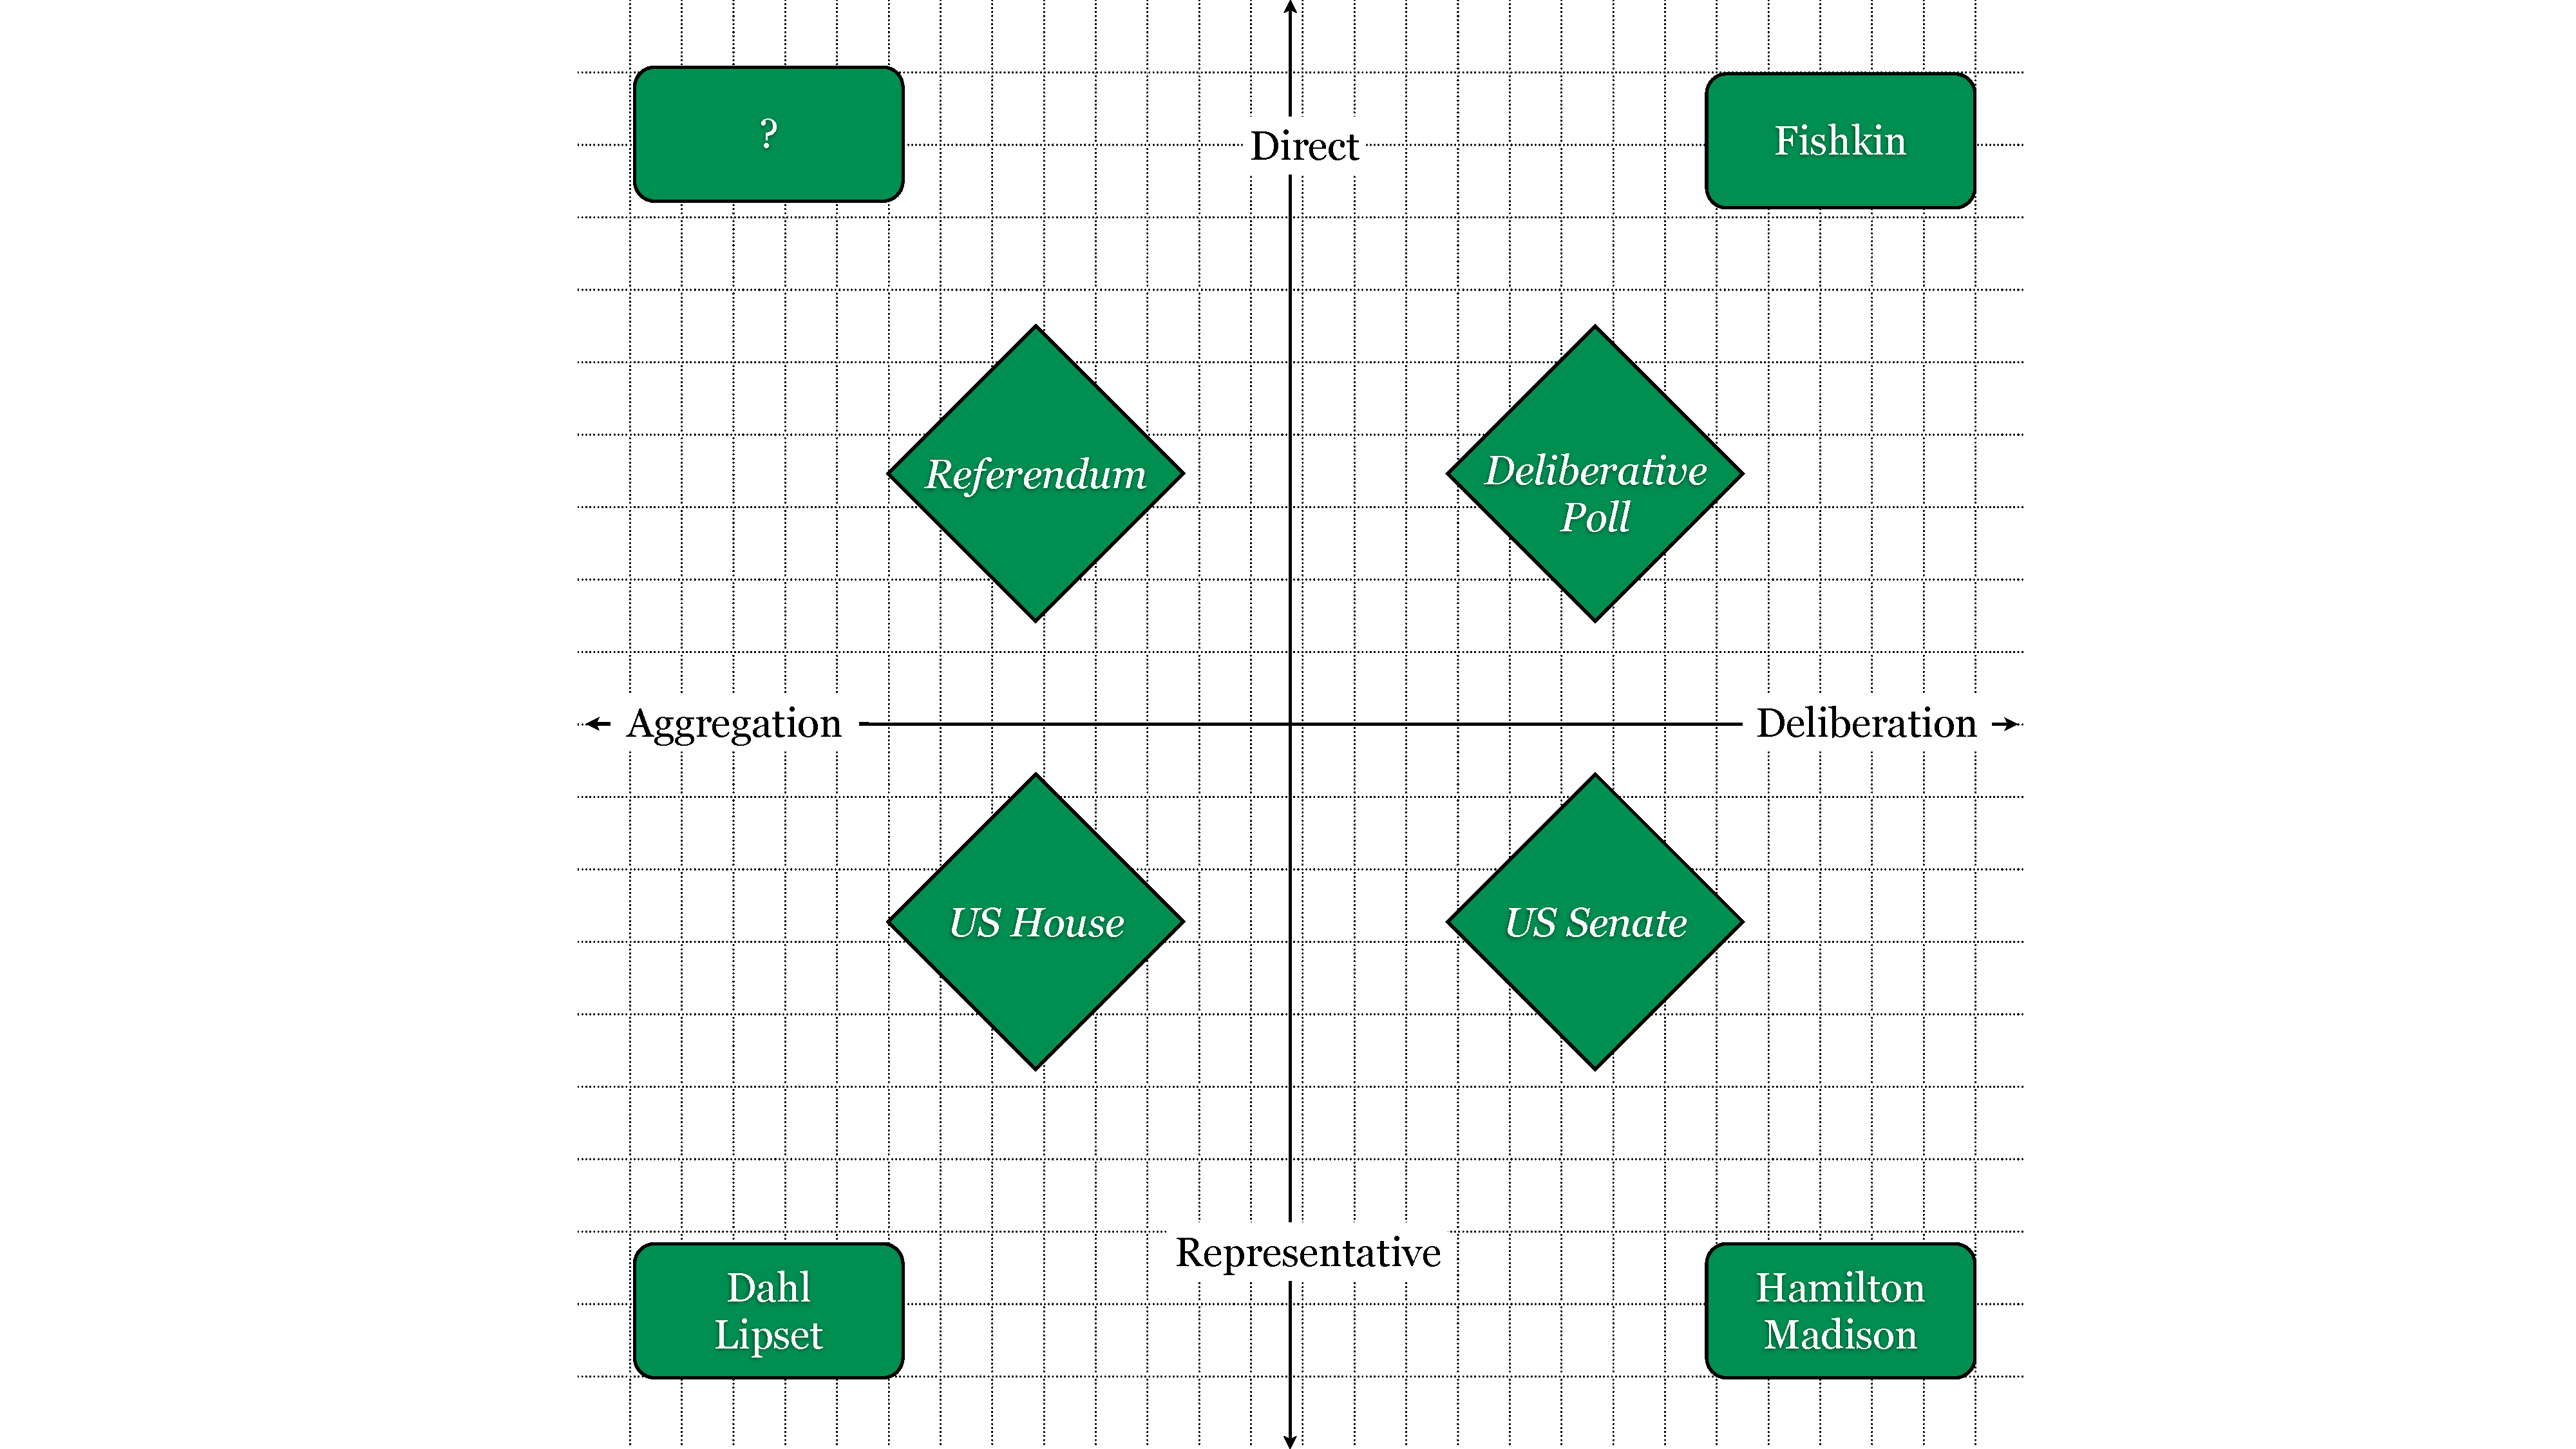
\includegraphics[width=1\linewidth]{democracy-2x2}
	\caption{Direct, Representative, Deliberative and Aggregative Democracy}
	\label{fig:democracy-2x2}
\end{figure}

\begin{figure}[htbp]
	\centering
	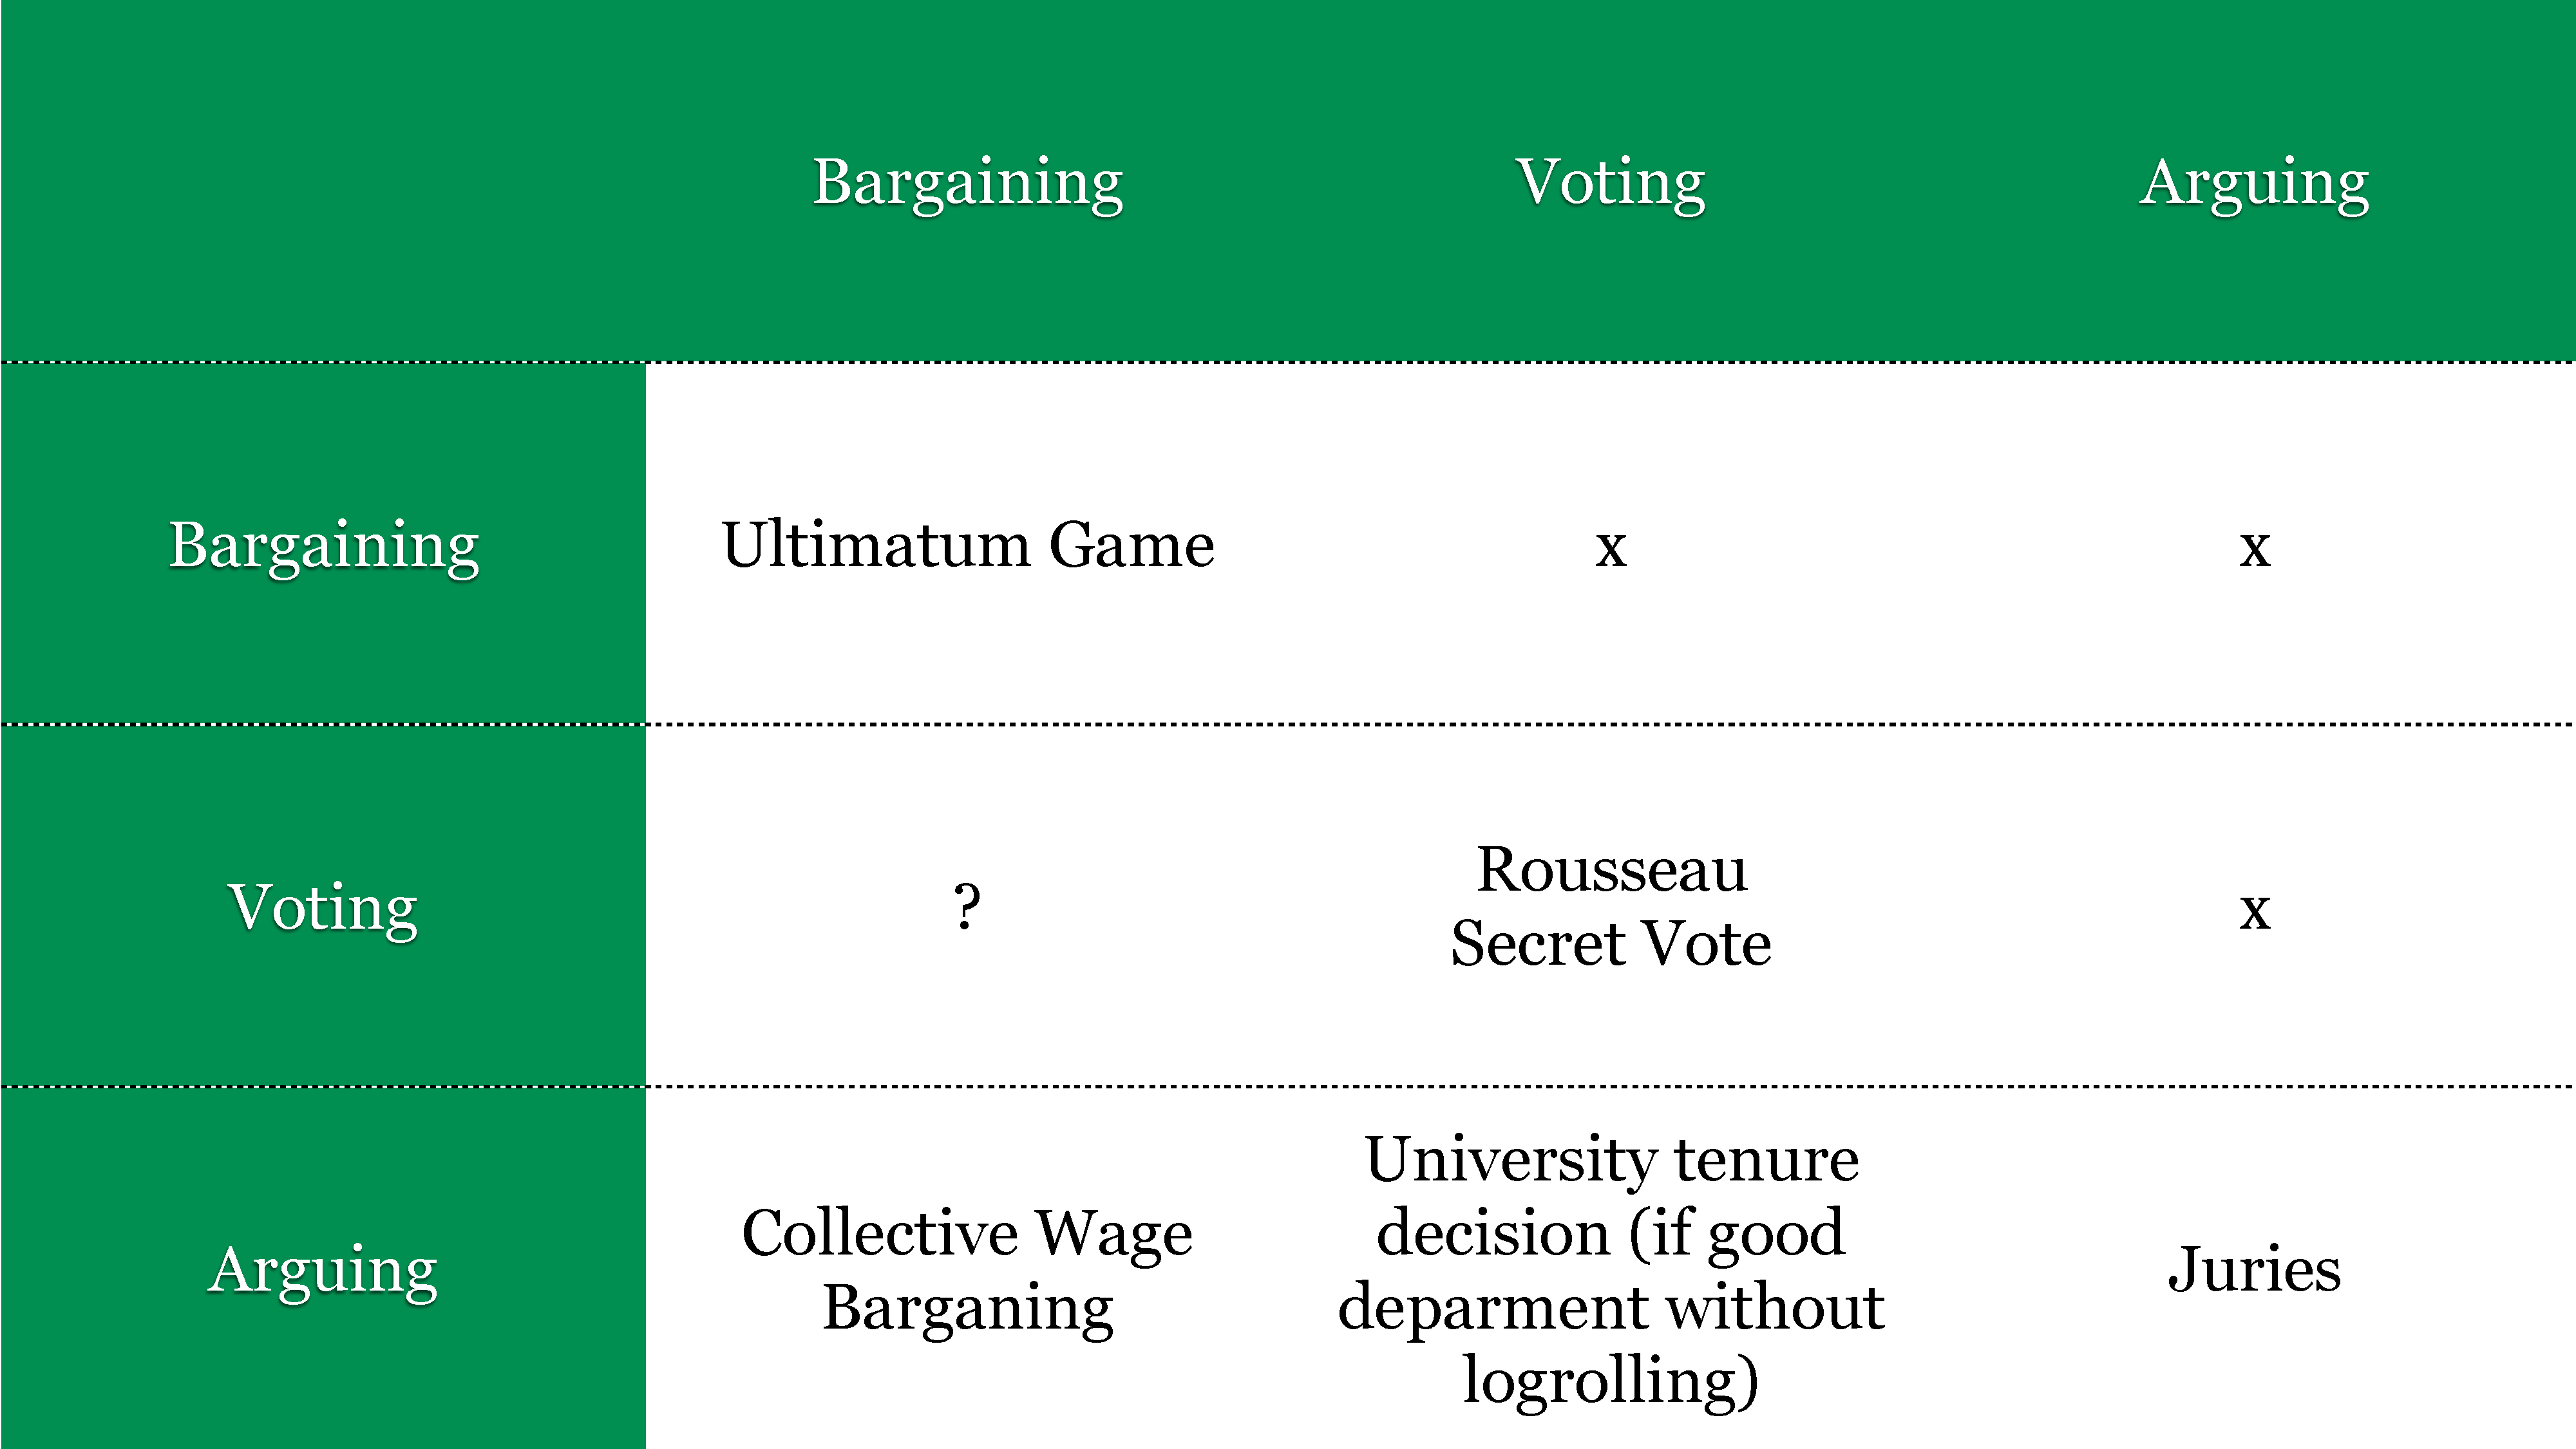
\includegraphics[width=1\linewidth]{democracy-3x3}
	\caption{Modes of Collective Decision Making}
	\label{fig:democracy-3x3}
\end{figure}

\section[Micropolitics]{The Micropolitics of Democracy}
%or political psychology?

\begin{quote}
	\emph{``The best argument against democracy is a five-minute talk with the average voter.''}
	\\*
	--- Winston Churchill (1874--1965)
\end{quote}


\subsection[Cognition]{Cognition}
		%People are cognitive misers (Kahneman + Tversky 1983)
		%cognition? (Rosenberg) %cognitive competence is key
		%Tversky and Kahnemann first attacked homo oeconomicus

\subsection[Behavior]{Behavioral Economics}
		%feature beahvioral econ somewhere, big
		%Link this to the big picture i'm drawing about this.

\subsection[Development]{Development}
		%	\chapter{Cognitive and Developmental Conditions of Deliberation}
		%Think Rousseau:

		%Emile, Piaget, Freud, Liberal Theory
		%Note that Rousseau wrote "Emile" and the Contrat Social.
		%Think Blinder + Lahmer, more of this is on Evernote

\subsection[Group Dynamics]{Group Dynamics}

\section[Macropolitics]{The Macropolitics of Democracy} %or public choice

\begin{quote}
	\emph{``I have about made up my mind that laws are like sausages ---
	the less you know about how they are made the more respect you have for them.''}
	\\*
	--- Otto von Bismarck (1815--1898)
\end{quote}

\begin{quote}
	\emph{``The stuck wheel gets the grease.''}
	\\*
	--- Unknown
\end{quote}

\subsection[Public Choice]{Public Choice aka Political Economy}
		%the set of institutions and dynamics building on homoeconomicus in the public realm and its dysfunctions
		%Bottom line
		%public choice ``markets'' fail, too
		%Who to turn to? \cite{Caplan2007} suggests, we should do more real market, instead of democracy
		%I don't think this works
		%It fails, so we have to turn to other modes, institutions (deliberations) that DO NOT build on homo oeconomicus.

		%Do sth on CAPLAN!

%add section on corruption and big money in politics (citizens united vs fed election commission)
%As TAL says, money never trump votes, but when people don't much care about an issue, money does matter
%That would be the majority of cases
%See:
%collective action Manson why some issues get represented, others not.
\subsubsection{Condorcet}
			%for example, (\citealt{Mankiw-2004-aa}:485)

\subsubsection{Arrow}
			%for example, (\citealt{Mankiw-2004-aa}:485)

\subsubsection{Median Voter}
			%for example, (\citealt{Mankiw-2004-aa}:485)

\subsubsection{Liberal Paradox}
			%get into this proof by Sen http://en.wikipedia.org/wiki/Liberal-paradox

\subsection[Effective Control]{Effective Control}

%from raes lecture on capitalism no 14 youtube
	%concentrated interests trump dispersed ones
	%well-financed interests trump poorly financed ones
	%defending the status quo is far easier than promoting change
	%agency capture is a big advantages
	%regulation may help those regulated more than it helps their putative victims